\documentclass[11pt,a4paper]{article}

\usepackage[utf8]{inputenc}
\usepackage[margin=1in]{geometry}
\usepackage{setspace}
\setstretch{1.15}
\usepackage{amsmath,amssymb,amsfonts,amsthm}
\usepackage{graphicx}
\usepackage{booktabs}
\usepackage{multirow}
\usepackage{array}
\usepackage{xcolor}
\usepackage{hyperref}
\usepackage{cite}
\usepackage{algorithm}
\usepackage{algpseudocode}
\usepackage{tikz}
\usetikzlibrary{shapes.geometric, arrows, positioning}
\usepackage{fancyhdr}
\usepackage{titlesec}
\usepackage{tocloft}

\hypersetup{
    colorlinks=true,
    linkcolor=black,
    citecolor=blue!70!black,
    urlcolor=blue!70!black
}

% Page numbering and header/footer settings
\pagestyle{fancy}
\fancyhf{}
\fancyhead[L]{\small\textit{RobustHFT-AgentLab: Mid-Term Project Report}}
\fancyhead[R]{\small\textit{NSUT, New Delhi}}
\fancyfoot[C]{\thepage}
\renewcommand{\headrulewidth}{0.4pt}
\renewcommand{\footrulewidth}{0.4pt}

\titleformat{\section}{\Large\bfseries\color{blue!80!black}}{\thesection}{1em}{}
\titleformat{\subsection}{\large\bfseries\color{blue!60!black}}{\thesubsection}{1em}{}
\titleformat{\subsubsection}{\normalsize\bfseries}{\thesubsubsection}{1em}{}

\begin{document}

% =============================================================================
% FRONT PAGE
% =============================================================================
\begin{titlepage}
    \centering
    \vspace*{0.5cm}
    
    {\LARGE \textbf{NETAJI SUBHAS UNIVERSITY OF TECHNOLOGY}}\\[0.3cm]
    {\large (Formerly Netaji Subhas Institute of Technology)}\\[0.2cm]
    {\normalsize Sector-3, Dwarka, New Delhi - 110078, India}\\[1.2cm]
    
    % University Logo / Graphic
    \IfFileExists{nsut_logo.png}{
        \includegraphics[width=3.5cm]{nsut_logo.png}\\[1.0cm]
    }{
        
\begin{tikzpicture}
            \draw[line width=1.5pt, color=blue!70!black] (0,0) circle (1.8cm);
            \draw[line width=0.8pt, color=blue!70!black] (0,0) circle (1.6cm);
            \node at (0, 0.4) [font=\bfseries\small, color=blue!80!black] {NSUT};
            \node at (0, -0.1) [font=\footnotesize, color=black] {ESTD. 1983};
            \node at (0, -0.6) [font=\tiny\bfseries, color=blue!70!black] {NEW DELHI};
        \end{tikzpicture}\\[1.0cm]
    }
    
    {\Large \textbf{MID-TERM PROJECT REPORT}}\\[0.4cm]
    {\large \textbf{Bachelor of Technology (B.Tech)}}\\[0.2cm]
    {\normalsize in Computer Science and Engineering}\\[1.2cm]
    
    \noindent\rule{\textwidth}{1.5pt}\\[0.4cm]
    {\LARGE \bfseries RobustHFT-AgentLab: Stress-Testing and Defending LLM Trading Agents Against Subtle Financial Misinformation}\\[0.3cm]
    {\large \textit{Temporal Grounding, Market Microstructure Evidence, and Execution Risk Controls}}\\[0.2cm]
    \noindent\rule{\textwidth}{1.5pt}\\[1.5cm]
    
    \begin{minipage}{0.45\textwidth}
        \begin{flushleft} \large
            \textbf{Submitted By:}\\[0.2cm]
            \textbf{[Student Name]}\\[0.1cm]
            Roll No: [Roll Number]\\[0.1cm]
            Department of CSE\\[0.1cm]
            NSUT, New Delhi
        \end{flushleft}
    \end{minipage}
    \hfill
    \begin{minipage}{0.45\textwidth}
        \begin{flushright} \large
            \textbf{Under the Guidance of:}\\[0.2cm]
            \textbf{[Supervisor Name]}\\[0.1cm]
            [Designation / Professor]\\[0.1cm]
            Department of CSE\\[0.1cm]
            NSUT, New Delhi
        \end{flushright}
    \end{minipage}
    
    \vfill
    {\large Academic Year: 2026--2027}\\[0.2cm]
    {\normalsize Department of Computer Science and Engineering}
\end{titlepage}

% =============================================================================
% TABLE OF CONTENTS
% =============================================================================
\newpage
\pagenumbering{roman}
\tableofcontents
\newpage
\pagenumbering{arabic}

% =============================================================================
% 1. INTRODUCTION
% =============================================================================
\section{Introduction}
\label{sec:introduction}

The deployment of Large Language Models (LLMs) in autonomous decision-making environments has rapidly transitioned from exploratory academic prototypes to high-stakes quantitative financial workflows. In algorithmic trading, recent frameworks such as FinMem~\cite{yu2025finmem}, FinCon~\cite{yu2024fincon}, and TradingAgents~\cite{xiao2025tradingagents} integrate generative language models into Partially Observable Markov Decision Process (POMDP) architectures. In these systems, an agent continuously observes quantitative market data (price histories, technical indicators, order metrics), retrieves textual market narratives (news reports, corporate filings, microblog feeds) from memory stores, and synthesizes multimodal signals to execute sequential financial decisions (Buy, Sell, or Hold).

While multimodal reasoning provides significant predictive flexibility, it simultaneously introduces a critical, asymmetric attack surface: \textbf{untrusted textual inputs}. Unlike numerical time series—which are strictly regulated and verified through consolidated market data feeds—textual news streams are decentralized, noisy, and highly susceptible to strategic injection. Traditional machine learning vulnerabilities, such as adversarial gradient perturbations or jailbreaking prompts, aim to bypass explicit safety boundaries to generate harmful language~\cite{jiang2024artprompt, zhou2025autoredteamer}. In contrast, financial misinformation operates under an entirely different paradigm: \textbf{subtle semantic distortion}. A malicious actor does not need to inject overtly false or toxic text. Instead, minor alterations—such as flipping a growth rate, inverting a qualitative sentiment descriptor, modifying an entity attribution, or subtly distorting causal claims—produce text that appears perfectly authentic, passes stylistic detection filters, and yet decisively manipulates the downstream trading policy~\cite{jiang2026glisters, yan2025tradetrap}.

\subsection{Base Paper Overview: AutoRedTrader}
The benchmark baseline for this project is \textit{AutoRedTrader: Autonomous Red Teaming of Trading Agents through Synthetic Misinformation Injection} (Liu et al., 2026, arXiv:2605.09185)~\cite{liu2026autoredtrader}. AutoRedTrader formalizes the autonomous red-teaming of LLM trading agents by defining a structured three-tiered operator space for generating synthetic financial misinformation:
\begin{enumerate}
    \item \textbf{Behavioral Bias Framing ($\Phi_{\text{Bias}}$):} Steering the target agent's psychological state through cognitive bias induction (e.g., triggering overconfidence, loss aversion, anchoring, or herding dynamics).
    \item \textbf{Minor Semantic Perturbations ($\Phi_{\text{Minor}}$):} Applying targeted atomic edits across eight distinct semantic categories, including directional flipping, sentiment inversion, numerical substitution, and causal swaps.
    \item \textbf{Style Rewriting ($\Phi_{\text{Rewrite}}$):} Camouflaging perturbed text into natural journalistic or formal financial research styles to evade surface-level linguistic filters.
\end{enumerate}
AutoRedTrader dynamically optimizes this perturbation space using a history-aware Pólya-urn reinforcement sampler, demonstrating that an autonomous attacker can flip trading decisions in up to 26.7\% of evaluated days. To counteract this, the authors propose a preliminary heuristic termed ``time-series-informed grounding.''

\subsection{Project Scope and Mid-Term Milestones}
This B.Tech Project, entitled \textbf{RobustHFT-AgentLab (`rhal`)}, develops an offline, deterministic, and academically rigorous defensive simulation laboratory that addresses the critical architectural and methodological vulnerabilities identified in existing literature. 

Rather than treating the problem as a single monolithic defense, this project designs a \textbf{Three-Tier Defense Hierarchy}:
\begin{itemize}
    \item \textbf{Tier 1: Admissible Temporal Grounding} — Historical analog retrieval and mathematical sentiment shrinkage with strict no-lookahead enforcement.
    \item \textbf{Tier 2: High-Frequency / Microstructure Evidence Fusion} — Incorporating fast-moving order-flow and spread proxies to ground textual claims in microscopic market reality.
    \item \textbf{Tier 3: Execution Risk-Control Layer} — Downstream portfolio safeguards (confidence gates, hold-on-conflict, volatility sizing, and drawdown throttling).
\end{itemize}

\textbf{Current Mid-Term Evaluation Status:} As of this mid-term evaluation, the baseline simulation platform and closed-loop MisGen red-teaming engine have been fully reproduced and mathematically verified. Furthermore, a major evaluation flaw in the base paper—namely, retrieval-induced noise—has been isolated through the implementation of a novel \textbf{Placebo Control Arm}. \textbf{Defense Tier 1 (Admissible Temporal Grounding) has been fully implemented}, and current work is actively focused on fine-tuning its coupling parameters ($\kappa$-shrinkage sweep) to map the optimal robustness-return Pareto frontier. Defenses Tier 2 and Tier 3, along with extensive cross-asset validations, form the scheduled deliverables for the final evaluation phase.

% =============================================================================
% 2. MOTIVATION
% =============================================================================
\section{Motivation}
\label{sec:motivation}

The motivation for this research stems from fundamental vulnerabilities discovered in the operation of autonomous LLM trading agents, alongside notable methodological deficiencies in the current state of the art.

\subsection{The Fragility of Textual Reliance in Quantitative Systems}
Quantitative finance has historically relied on strict statistical models operating on price, volume, and order-book state. The introduction of LLMs has democratized unstructured text interpretation, enabling agents to parse real-time breaking news. However, LLMs lack an intrinsic understanding of physical or financial reality; they process text probabilistically based on linguistic token associations. Consequently, when an agent encounters synthetic narratives that mimic genuine financial press releases, it suffers from cognitive capture: the textual signal completely overrides the quantitative reality. In backtests, an agent fed manipulated earnings reports or fabricated executive statements consistently misallocates capital, resulting in catastrophic portfolio drawdowns.

\subsection{Methodological Flaws Identified in the Base Paper}
A critical study of the base paper (\textit{AutoRedTrader}) revealed four major limitations that undermine its real-world applicability and empirical conclusions:

\begin{enumerate}
    \item \textbf{The Retrieval Confound: Failure to Disentangle Attack Semantics from Retrieval Noise.}
    In existing studies, the Attack Success Rate (ASR) is computed by comparing a clean execution run against an injected run. However, the retrieval mechanism relies on top-$k$ similarity matching over a dynamically updated document pool. Adding synthetic documents—irrespective of their semantic content—naturally alters document rank ordering, displacing marginal clean articles. In near-threshold market regimes, minor changes in retrieved context flip decisions purely due to \textit{retrieval noise}. AutoRedTrader failed to isolate this effect, leading to over-reported attack efficacy.
    
    \item \textbf{Temporal Lookahead Leakage in Historical Analog Grounding.}
    The grounding mechanism in AutoRedTrader searches past market windows to validate current news. However, in their mathematical formulation, an analog identified at historical time $e$ with forward outcome horizon $H$ is considered valid even when $e < t$. If $e + H > t$, the analog's outcome window overlaps with future data relative to $t$, creating subtle lookahead leakage that invalidates the backtest.
    
    \item \textbf{Coarse Macro Indicators vs. Microscopic Market Reality.}
    Existing temporal grounding relies exclusively on coarse, low-frequency daily indicators (e.g., 5-day return, 20-day volatility). Real-world markets reflect institutional activity at the microstructure level. A textual release claiming ``overwhelming institutional accumulation'' can be immediately falsified if high-frequency Order-Flow Imbalance (OFI) is negative and bid-ask spreads are widening. Neglecting microstructure leaves the defense blind to intraday order book reality.
    
    \item \textbf{Absence of Downstream Portfolio Risk Management.}
    In quantitative finance, no signal is executed without risk filtration. The base paper assumes raw agent decisions directly dictate market execution. In practice, a robust defense requires execution-level circuit breakers that override decisions whenever textual confidence and market consistency diverge.
\end{enumerate}

These gaps provide the direct impetus for our three-tier defensive architecture and rigorous paired evaluation framework.

% =============================================================================
% 3. LITERATURE SURVEY
% =============================================================================
\section{Literature Survey}
\label{sec:literature_survey}

The intersection of generative artificial intelligence, adversarial robustness, and quantitative financial engineering spans several distinct research domains. A structured review of the relevant literature is organized below.

\subsection{LLM-Based Financial Trading Agents}
The paradigm of utilizing language models as sequential financial agents originated with FinMem~\cite{yu2025finmem}, which established layered memory structures (working memory and long-term episodic memory) alongside character profiles to simulate cognitive investment behavior. Li et al.~\cite{li2025investorbench} introduced InvestorBench, formalizing the standard POMDP trading agent architecture divided into four functional modules: Perception (data parsing), Profile (risk and style alignment), Memory (retrieval-augmented storage), and Action (execution synthesis). FinCon~\cite{yu2024fincon} extended this with multi-agent conceptual verbal reinforcement, where specialized analyst agents debate trade validity. TradingAgents~\cite{xiao2025tradingagents} and FinAgent~\cite{zhang2024finagent} introduced tool-augmented planning and multimodal observation capabilities. While these systems demonstrate superior alpha generation in benign market conditions, none were evaluated against intentional, adversarial informational corruption.

\subsection{Adversarial Vulnerabilities and Financial Red-Teaming}
Adversarial attacks against NLP systems historically focused on character or token-level substitutions (e.g., TextFooler, HotFlip) or adversarial prefix prompts designed to elicit toxic output~\cite{jiang2024artprompt, zhou2025autoredteamer}. In financial contexts, Yan et al. introduced TradeTrap~\cite{yan2025tradetrap}, demonstrating that state-of-the-art LLMs (including GPT-4 and Claude-3) exhibit significant decision instability when exposed to minor prompt paraphrasing. Wang et al.~\cite{wang2026life} characterized prompt-induced linguistic fingerprints in machine-generated news, noting that subtle stylistic adaptations can easily evade static discriminators. Jiang et al.~\cite{jiang2026glisters} developed GLISTERS, a benchmark for reference-free counterfactual financial misinformation detection, proving that detecting semantic inversion without access to the ground-truth event is near chance level for standard classifiers. AutoRedTrader~\cite{liu2026autoredtrader} consolidated these insights into an automated red-teaming loop specifically optimized to force agent action flips.

\subsection{Behavioral Finance and Cognitive Biases}
Behavioral economics establishes that human traders systematically deviate from rational expectations. Barber and Odean~\cite{barber2001boys} documented how overconfidence leads to excessive trading and reduced risk aversion. Kahneman and Tversky's Prospect Theory~\cite{kahneman2013prospect} established loss aversion—the psychological asymmetry where losses are felt roughly twice as intensely as equivalent gains. Spyrou~\cite{spyrou2013herding} analyzed herding behaviors where market participants discard private information to follow collective consensus, while De Long et al.~\cite{delong1990noise} proved that noise traders driven by cognitive heuristics can create persistent price anomalies. These psychological biases serve as the mathematical foundation for adversarial framing operators ($\Phi_{\text{Bias}}$) that exploit the inductive biases of LLMs.

\subsection{Market Microstructure and Backtest Integrity}
High-frequency market microstructure offers empirical proxies that capture supply-demand asymmetries before they manifest in closing prices. Corwin and Schultz~\cite{corwin2012spread} derived a robust high-low estimator for effective bid-ask spreads. Garman and Klass~\cite{garman1980estimation} developed an extremely efficient realized volatility estimator using extreme value distributions. Cont, Kukanov, and Stoikov~\cite{cont2014price} proved that Order-Flow Imbalance (OFI)—the net imbalance between buying and selling volume at the best quotes—exhibits a near-linear instantaneous relationship with price change. Amihud's illiquidity measure~\cite{amihud2002illiquidity} quantifies the price impact per unit of trading volume. Finally, in backtest methodology, Bailey et al.~\cite{bailey2014probability} and López de Prado~\cite{lopezdeprado2018advances} emphasized that lookahead bias and selection bias are the primary causes of backtest failure, mandating strictly causal, trailing data transformations.

\begin{table}[htbp]
\centering
\caption{Comparative Analysis: Existing Literature vs. RobustHFT-AgentLab (`rhal`)}
\label{tab:lit_comparison}
\resizebox{\textwidth}{!}{
\begin{tabular}{lcccccc}
\toprule
\textbf{Framework / System} & \textbf{Agent Architecture} & \textbf{Adversarial Loop} & \textbf{Grounding Method} & \textbf{Microstructure Proxies} & \textbf{Risk Controls} & \textbf{Placebo / Net ASR} \\
\midrule
FinMem (2025)~\cite{yu2025finmem} & POMDP + Layered Memory & None & None & None & None & No \\
TradeTrap (2025)~\cite{yan2025tradetrap} & Single LLM Prompt & Static Paraphrasing & None & None & None & No \\
AutoRedTrader (2026)~\cite{liu2026autoredtrader} & Memory-Augmented LLM & Closed-Loop (Pólya-Urn) & Daily Indicators ($e < t$) & None & None & No (Naive ASR only) \\
\midrule
\textbf{RobustHFT-AgentLab (Ours)} & \textbf{Modular POMDP} & \textbf{Closed-Loop (Pólya-Urn)} & \textbf{Admissible ($e+H \le t$)} & \textbf{OFI, Spread, GK-RV} & \textbf{Multi-Barrier Risk} & \textbf{Yes (Paired Net ASR)} \\
\bottomrule
\end{tabular}
}
\end{table}

% =============================================================================
% 4. PROBLEM STATEMENT
% =============================================================================
\section{Problem Statement}
\label{sec:problem_statement}

Let an autonomous financial trading agent operate within a discrete-time financial market over a trading horizon $t \in \{1, 2, \dots, T\}$. At each step $t$, the agent receives an observation tuple:
\begin{equation}
    o_t = \left( \mathbf{x}_{1:t}, \mathcal{D}_t \right)
\end{equation}
where $\mathbf{x}_{1:t} \in \mathbb{R}^{t \times d}$ denotes the strictly causal historical market time series (OHLCV prices and derived technical indicators), and $\mathcal{D}_t = \{d_1, d_2, \dots, d_k\}$ is a retrieved subset of $k$ news documents obtained from a memory pool $\mathcal{M}_t$.

The agent maintains an internal state $s_t$ composed of its perception of market conditions, its behavioral profile context $\mathbf{b}$, and episodic memory traces. The policy $\pi_\theta(a_t \mid o_t, s_t)$ maps observations to discrete portfolio actions:
\begin{equation}
    a_t \in \{\text{Buy } (+1), \text{Hold } (0), \text{Sell } (-1)\}
\end{equation}

\subsection{Threat Model: Closed-Loop Misinformation Injection}
An external red-team adversary seeks to induce erroneous trading decisions by perturbing the information environment. The adversary cannot modify the consolidated market data $\mathbf{x}_{1:t}$ (which is secured by exchange protocols), nor can it directly alter the model parameters $\theta$. The adversary's sole attack vector is injecting a synthetic document $d^*_t$ into the unverified news repository $\mathcal{M}_t$.

To be effective and evade security tripwires, $d^*_t$ must satisfy two conflicting constraints:
\begin{enumerate}
    \item \textbf{Evasion (Plausibility):} $d^*_t$ must closely resemble genuine financial reporting. It must pass a semantic similarity filter $A_{\text{sim}}(d^*_t, d_t) \ge \tau_{\text{sim}}$ and a linguistic detectability filter $A_{\text{det}}(d^*_t) \le \tau_{\text{det}}$.
    \item \textbf{Efficacy (Decision Flipping):} When retrieved into $\mathcal{D}_t$, $d^*_t$ must alter the agent's action relative to its unperturbed decision: $a_t^{\text{injected}} \ne a_t^{\text{clean}}$.
\end{enumerate}

\subsection{Formalization of Evaluation Metrics}
A central flaw of previous research is evaluating attacks using naive Attack Success Rate. We formally define the metric space to eliminate retrieval confounds:

\begin{itemize}
    \item \textbf{Naive Attack Success Rate (ASR):} The fraction of trading days where the attacked agent's decision diverges from the shadow clean agent:
    \begin{equation}
        \text{ASR} = \frac{1}{T} \sum_{t=1}^T \mathbb{I}\left( a_t^{\text{treated}} \ne a_t^{\text{clean}} \right)
    \end{equation}
    
    \item \textbf{Placebo ASR ($\text{ASR}_{\text{placebo}}$):} The fraction of decision flips observed when the agent is exposed to a placebo pool $\mathcal{M}_t^{\text{placebo}}$, where synthetic documents are strictly meaning-preserving paraphrases ($\Phi_{\text{Placebo}}$) carrying zero adversarial distortion:
    \begin{equation}
        \text{ASR}_{\text{placebo}} = \frac{1}{T} \sum_{t=1}^T \mathbb{I}\left( a_t^{\text{placebo}} \ne a_t^{\text{clean}} \right)
    \end{equation}
    
    \item \textbf{Net Attack Success Rate ($\text{ASR}_{\text{net}}$):} The true, semantically attributable attack efficacy, isolating the causal effect of misinformation from retrieval pool reshuffling:
    \begin{equation}
        \text{ASR}_{\text{net}} = \max\left(0, \, \text{ASR}_{\text{injected}} - \text{ASR}_{\text{placebo}}\right)
    \end{equation}
    
    \item \textbf{Misinformation Exposure Rate (MER) and Lift:} The proportion of retrieved documents that are synthetic, compared against the background synthetic base rate:
    \begin{equation}
        \text{MER} = \frac{1}{T \cdot k} \sum_{t=1}^T \sum_{i=1}^k \mathbb{I}\left( d_{t,i} \in \mathcal{M}_{\text{synthetic}} \right), \quad \text{MER Lift} = \frac{\text{MER}}{\text{Base Rate}_{\text{synthetic}}}
    \end{equation}
\end{itemize}

The core problem is designing a defense mechanism that minimizes $\text{ASR}_{\text{net}}$ and drawdown under adversarial injection, while preserving the baseline cumulative return (CR) and Sharpe ratio in clean environments.

% =============================================================================
% 5. OBJECTIVE AND METHODOLOGY
% =============================================================================
\section{Objective and Methodology}
\label{sec:objective_and_methodology}

\subsection{Core Objectives}
\begin{enumerate}
    \item \textbf{Phase 1 (Mid-Term Completed):} Construct an end-to-end, offline, CPU-only simulation testbed replicating the closed-loop AutoRedTrader framework; establish a paired shadow evaluation methodology with a placebo arm; fully implement and unit-test \textbf{Defense Tier 1: Admissible Temporal Grounding}.
    \item \textbf{Phase 1 Ongoing (Mid-Term Tuning):} Calibrate the grounding coupling parameter $\kappa \in [0.3, 1.0]$ to quantify the Pareto frontier between attack resistance and clean return preservation.
    \item \textbf{Phase 2 (End-Term Scheduled):} Formulate and integrate \textbf{Defense Tier 2: High-Frequency / Microstructure Evidence Fusion} (Garman-Klass RV, Corwin-Schultz spread, and Order-Flow Imbalance).
    \item \textbf{Phase 3 (End-Term Scheduled):} Implement \textbf{Defense Tier 3: Execution Risk-Control Layer} (Hold-on-Conflict, volatility sizing, and drawdown circuit breakers), followed by full multi-seed ablation and real-market data testing.
\end{enumerate}

\subsection{System Architecture}
The framework operates as an integrated closed-loop pipeline depicted in Figure~\ref{fig:architecture}. Every component is governed by strict deterministic seeding, eliminating stochastic divergence across paired comparisons.

\begin{figure}[htbp]
\centering
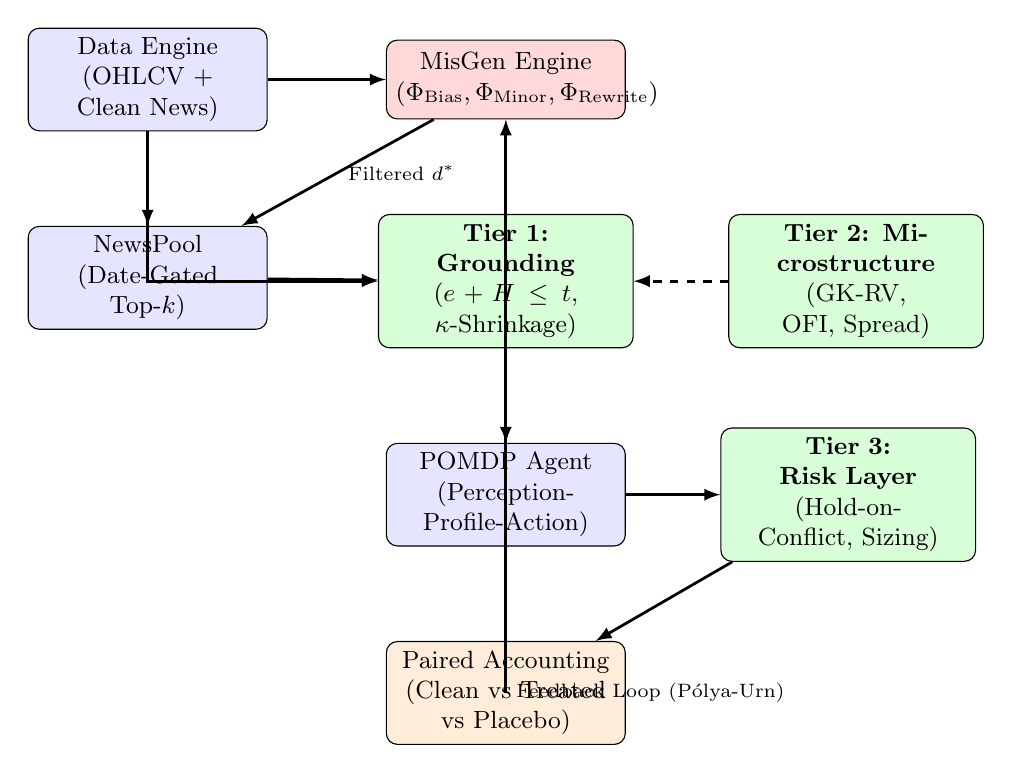
\begin{tikzpicture}[node distance=1.3cm, auto, >=latex]
    \tikzstyle{block} = [rectangle, draw, fill=blue!10, text width=2.8cm, text centered, rounded corners, minimum height=1.0cm, font=\small]
    \tikzstyle{defblock} = [rectangle, draw, fill=green!15, text width=3.0cm, text centered, rounded corners, minimum height=1.0cm, font=\small]
    \tikzstyle{attackblock} = [rectangle, draw, fill=red!15, text width=2.8cm, text centered, rounded corners, minimum height=1.0cm, font=\small]
    \tikzstyle{evalblock} = [rectangle, draw, fill=orange!15, text width=2.8cm, text centered, rounded corners, minimum height=1.0cm, font=\small]

    \node [block] (market) {Data Engine\\(OHLCV + Clean News)};
    \node [attackblock, right=1.5cm of market] (misgen) {MisGen Engine\\($\Phi_{\text{Bias}}, \Phi_{\text{Minor}}, \Phi_{\text{Rewrite}}$)};
    \node [block, below=1.2cm of market] (memory) {NewsPool\\(Date-Gated Top-$k$)};
    \node [defblock, below=1.2cm of misgen] (grounding) {\textbf{Tier 1: Grounding}\\($e+H \le t$, $\kappa$-Shrinkage)};
    \node [defblock, right=1.2cm of grounding] (micro) {\textbf{Tier 2: Microstructure}\\(GK-RV, OFI, Spread)};
    \node [block, below=1.2cm of grounding] (agent) {POMDP Agent\\(Perception-Profile-Action)};
    \node [defblock, right=1.2cm of agent] (risk) {\textbf{Tier 3: Risk Layer}\\(Hold-on-Conflict, Sizing)};
    \node [evalblock, below=1.2cm of agent] (eval) {Paired Accounting\\(Clean vs Treated vs Placebo)};

    \draw[->, line width=1pt] (market) -- (misgen);
    \draw[->, line width=1pt] (market) -- (memory);
    \draw[->, line width=1pt] (misgen) -- node[right, font=\scriptsize]{Filtered $d^*$} (memory);
    \draw[->, line width=1pt] (memory) -- (grounding);
    \draw[->, line width=1pt] (market) |- (grounding);
    \draw[->, line width=1pt, dashed] (micro) -- (grounding);
    \draw[->, line width=1pt] (grounding) -- (agent);
    \draw[->, line width=1pt] (agent) -- (risk);
    \draw[->, line width=1pt] (risk) -- (eval);
    \draw[->, line width=1pt] (eval) -| node[pos=0.25, right, font=\scriptsize]{Feedback Loop (Pólya-Urn)} (misgen);
\end{tikzpicture}
\caption{RobustHFT-AgentLab closed-loop simulation architecture, highlighting the 3-Tier Defense Hierarchy and paired evaluation harness.}
\label{fig:architecture}
\end{figure}

\subsection{The 3-Tier Defense Hierarchy}

\subsubsection{Tier 1: Admissible Temporal Grounding (Implemented \& In Tuning)}
Temporal grounding reconciles textual news claims with quantitative price patterns. When news is retrieved at step $t$, the grounding engine queries historical market windows of duration $W=30$ days to identify historical analogs matching the current market state $\mathbf{x}_{t-W:t}$.

\textbf{The Mathematical Admissibility Constraint:} To prevent lookahead leakage, every historical candidate window starting at $s$ and ending at $e = s + W$ with forward evaluation horizon $H = 5$ days must satisfy:
\begin{equation}
    e + H \le t
\end{equation}
If an analog satisfies this condition, its realized forward market outcome $\Delta p_{e \to e+H}$ is strictly in the historical past relative to decision time $t$. The top-$K$ analogs are retrieved via Euclidean distance over normalized feature vectors, yielding an expected analog return $r_{\text{analog}}$ and confidence $c \in [0, 1]$.

\textbf{Sentiment Shrinkage Formula:} Let $s_{\text{raw}} \in [-1, 1]$ be the raw sentiment score extracted from retrieved news, and $s_{\text{mkt}} = \text{sign}(r_{\text{analog}}) \cdot \min(1, |r_{\text{analog}}|/\sigma)$ be the market-implied sentiment. The grounded sentiment $s_g$ is formulated as a shrinkage estimator:
\begin{equation}
    s_g = s_{\text{raw}} - \kappa \cdot (1 - c) \cdot \left( s_{\text{raw}} - s_{\text{mkt}} \right)
\end{equation}
where $\kappa \in [0, 1]$ is the grounding strength parameter. When text and market evidence conflict and confidence $c$ is low, $\kappa$ pulls the effective sentiment toward market reality. We are currently performing a rigorous empirical sweep of $\kappa \in \{0.3, 0.7, 1.0\}$.

\subsubsection{Tier 2: High-Frequency / Microstructure Proxies (Formulated for End-Term)}
While Tier 1 operates on daily OHLCV bars, Tier 2 equips the grounding layer with high-frequency microstructure estimators:
\begin{itemize}
    \item \textbf{Garman-Klass Realized Volatility ($GK\text{-}RV$):} Captures intraday price dynamics using open ($O$), high ($H$), low ($L$), and close ($C$):
    \begin{equation}
        \sigma_{GK}^2 = 0.511 \left(\ln \frac{H}{C}\right)^2 - 0.019 \left[\ln \frac{C}{O} \ln \frac{H \cdot L}{O^2} - 2 \ln \frac{H}{O} \ln \frac{L}{O}\right] - 0.383 \left(\ln \frac{C}{O}\right)^2
    \end{equation}
    \item \textbf{Corwin-Schultz Spread Proxy ($S$):} Estimates bid-ask spread from 2-day high-low price ratios, capturing liquidity dry-ups.
    \item \textbf{Order-Flow Imbalance Proxy ($OFI$):} Approximates net order pressure using volume and the sign of intraday price changes:
    \begin{equation}
        OFI_t = \text{Vol}_t \cdot \frac{2 C_t - H_t - L_t}{H_t - L_t}
    \end{equation}
\end{itemize}
In Phase 2, these proxies will be fused into the state vector, allowing the agent to detect when bullish text is contradicted by order book liquidity withdrawal.

\subsubsection{Tier 3: Execution Risk-Control Layer (Formulated for End-Term)}
The final defense tier operates downstream of the agent's policy $\pi_\theta$, enforcing strict portfolio risk boundaries:
\begin{itemize}
    \item \textbf{Hold-on-Conflict Filter:} If the sign of the textual sentiment contradicts the market trend ($\text{sign}(s_{\text{raw}}) \ne \text{sign}(s_{\text{mkt}})$) and confidence is below threshold $\tau_{\text{conf}}$, the action is forced to Hold ($a_t = 0$).
    \item \textbf{Volatility-Targeted Sizing:} Position size is scaled inversely with Garman-Klass volatility: $w_t = \min\left(1.0, \frac{\sigma_{\text{target}}}{\sigma_{GK, t}}\right)$.
    \item \textbf{Drawdown Circuit Breaker:} If trailing portfolio drawdown exceeds $\text{DD}_{\text{max}} = 5\%$, all trading is halted until volatility normalizes.
\end{itemize}

\subsection{Adversarial Generation and Closed-Loop Steering}
The MisGen engine generates candidate perturbations across three spaces:
\begin{equation}
    d^* = \Phi_{\text{Rewrite}}\left( \Phi_{\text{Minor}}\left( d, \Phi_{\text{Bias}}(\mathbf{b}) \right) \right)
\end{equation}
Candidate documents are passed through a TF-IDF cosine similarity gate ($A_{\text{sim}} \ge 0.35$) and our trained logistic detectability proxy ($A_{\text{det}} \le \tau_{\text{det}}$). Surviving documents enter the pool. 

To steer the attack online, the adversary samples operator combinations $(b, m, r)$ using a generalized Pólya-urn model. Let $w_{b,m,r}^{(t)}$ be the weight of an operator tuple at step $t$. When an injected document successfully flips an agent's decision ($a_t^{\text{injected}} \ne a_t^{\text{clean}}$), its weight is reinforced:
\begin{equation}
    w_{b,m,r}^{(t+1)} = w_{b,m,r}^{(t)} + \alpha \cdot \mathbb{I}(\text{flip}_t) + \delta \cdot |\Delta \text{Return}_t|
\end{equation}
where $\alpha=1.0$ is the discrete flip bonus and $\delta=0.15$ rewards return destruction.

% =============================================================================
% 6. SIMULATION PLATFORM AND REQUIREMENTS
% =============================================================================
\section{Simulation Platform and Requirements}
\label{sec:simulation_platform}

\subsection{Software and Hardware Specifications}
To ensure universal academic reproducibility without dependency on paid commercial APIs or dedicated GPU clusters, the platform is engineered under strict design specifications:
\begin{itemize}
    \item \textbf{Operating Environment:} macOS (Darwin 24.3.0 / Apple Silicon) and Linux (Ubuntu 22.04+).
    \item \textbf{Programming Language:} Python 3.14 (fully compatible with Python 3.10+).
    \item \textbf{Core Libraries:} NumPy 2.5 (vectorized numerical computing), Pandas 3.0 (time series alignment), Scikit-Learn 1.9 (detectability modeling and TF-IDF vectorization), Pytest 8.0+ (regression and invariant test harness).
    \item \textbf{Documentation \& Typesetting:} TeX Live / Tectonic (automated offline IEEE report generation).
    \item \textbf{Hardware Constraints:} 100\% CPU-only execution; maximum memory footprint $< 1.5$ GB RAM; execution time for a full 5-seed, 9-arm simulation $< 60$ seconds.
\end{itemize}

\subsection{Safety Boundaries and Provenance Enforcement}
To guarantee that synthetic misinformation remains strictly quarantined within the simulation sandbox, the data architecture enforces structural safety controls:
\begin{itemize}
    \item Every generated document schema explicitly mandates a metadata tag: \texttt{provenance = "synthetic"} or \texttt{provenance = "placebo"}.
    \item The simulation platform contains no broker connectors, no order routing hooks, and no public dissemination interfaces.
    \item Market data loaders operate in read-only mode over synthetic GARCH processes or cached local historical CSVs.
\end{itemize}

\subsection{Structural No-Lookahead Architecture and Verification}
A primary technical contribution is the mathematical verification of no-lookahead guarantees. Financial backtests are notoriously prone to subtle data snooping (e.g., standardizing using full-sample means or executing at the closing price of the signal day). In RobustHFT-AgentLab:
\begin{enumerate}
    \item \textbf{Next-Open Execution:} Decisions synthesized at the close of day $t$ using information $\mathcal{I}_t$ are executed strictly at the opening price of day $t+1$ ($\text{Open}_{t+1}$), incorporating a 5 bps transaction fee and 5 bps linear slippage penalty.
    \item \textbf{Trailing Normalization:} All feature z-scores and rolling volatilities use trailing rolling windows strictly terminated at $t$.
    \item \textbf{Future-Mutation Test Harness:} The platform includes an automated unit test suite (\texttt{tests/test\_features\_nolookahead.py}). The test records the agent's feature values and trading decisions at historical step $t$, artificially mutates the market data for all steps $t' > t$ with random noise, and re-executes the pipeline. The test mathematically asserts that past decisions and representations remain bitwise identical, proving zero future leakage.
\end{enumerate}

\subsection{Preliminary Mid-Term Experimental Results}
The baseline reproduction, placebo arm, and Tier 1 grounding have been executed across 5 independent random seeds ($42, 43, 44, 45, 46$) over a 60-day active trading period (preceded by a 250-day analog warm-up history). The preliminary experimental results are summarized in Table~\ref{tab:preliminary_results}.

\begin{table}[htbp]
\centering
\caption{Preliminary Experimental Results Across 5 Seeds (Mean $\pm$ Std. Dev.)}
\label{tab:preliminary_results}
\resizebox{\textwidth}{!}{
\begin{tabular}{lcccccc}
\toprule
\textbf{Experimental Arm} & \textbf{MER (\%)} & \textbf{MER Lift} & \textbf{Naive ASR (\%)} & \textbf{Net ASR (\%)} & \textbf{Clean Return (\%)} & \textbf{Max Drawdown (\%)} \\
\midrule
\texttt{clean\_\_none} (Undefended Baseline) & $0.0 \pm 0.0$ & $0.00 \times$ & $0.0 \pm 0.0$ & --- & $+4.3 \pm 5.7$ & $-4.9 \pm 1.5$ \\
\texttt{placebo\_\_none} (Noise Control Arm) & $50.7 \pm 0.8$ & $1.03 \times$ & $21.3 \pm 4.4$ & --- & $+3.3 \pm 4.4$ & $-4.7 \pm 2.4$ \\
\texttt{injected\_\_none} (Attacked Baseline) & $63.4 \pm 2.2$ & $1.30 \times$ & $\mathbf{35.0 \pm 6.4}$ & $\mathbf{13.7 \pm 6.4}$ & $+5.6 \pm 5.7$ & $-3.5 \pm 1.1$ \\
\midrule
\texttt{clean\_\_grounded} (Tier 1 Defense Clean) & $0.0 \pm 0.0$ & $0.00 \times$ & $0.0 \pm 0.0$ & --- & $-0.8 \pm 2.7$ & $-4.9 \pm 1.2$ \\
\texttt{placebo\_\_grounded} (Tier 1 Placebo) & $50.4 \pm 0.6$ & $1.03 \times$ & $15.7 \pm 7.0$ & --- & $-1.4 \pm 4.3$ & $-5.5 \pm 0.1$ \\
\texttt{injected\_\_grounded} (Tier 1 Attacked, $\kappa=0.7$) & $61.3 \pm 3.5$ & $1.26 \times$ & $\mathbf{21.7 \pm 4.7}$ & $\mathbf{6.0 \pm 7.2}$ & $-1.3 \pm 5.0$ & $-5.8 \pm 2.3$ \\
\bottomrule
\end{tabular}
}
\end{table}

\textbf{Key Mid-Term Findings:}
\begin{enumerate}
    \item \textbf{Validation of the Placebo Discovery:} In the undefended agent, naive ASR is $35.0\%$. However, exposing the agent to meaning-preserving placebo text flips decisions in $21.3\%$ of days purely due to retrieval pool reshuffling! Consequently, the true adversarial semantic impact ($\text{ASR}_{\text{net}}$) is $13.7\%$, proving that prior literature significantly overstated attack potency by omitting retrieval controls.
    \item \textbf{Efficacy of Tier 1 Grounding:} Implementing Admissible Temporal Grounding reduces naive ASR from $35.0\%$ to $21.7\%$ (a $13.3$ percentage point absolute reduction) and slashes $\text{ASR}_{\text{net}}$ from $13.7\%$ to $6.0\%$ (a $56.2\%$ relative reduction in net attack vulnerability).
    \item \textbf{Current Work — Calibrating the $\kappa$-Frontier:} Our active tuning sweep shows that while $\kappa=0.7$ provides substantial attack suppression, it introduces a mild conservative drag on clean returns (from $+4.3\%$ to $-0.8\%$). Calibrating $\kappa$ across the spectrum $[0.3, 1.0]$ is currently underway to identify the Pareto-optimal configuration before layering Tier 2 and Tier 3 defenses.
\end{enumerate}

% =============================================================================
% 7. CONCLUSION
% =============================================================================
\section{Conclusion}
\label{sec:conclusion}

\subsection{Summary of Mid-Term Achievements}
At this mid-term evaluation stage, the project has successfully accomplished its foundational technical objectives:
\begin{itemize}
    \item \textbf{Robust Testbed Reproduction:} Replicated the closed-loop red-teaming framework of AutoRedTrader within an offline, fully deterministic, CPU-only simulation environment supported by a passing 62-test verification suite.
    \item \textbf{Methodological Breakthrough:} Formalized and validated the \textbf{Placebo Control Arm}, demonstrating that $21.3\%$ of observed decision flips in existing benchmarks stem from retrieval displacement rather than semantic deception, establishing $\text{ASR}_{\text{net}}$ as the mandatory metric for financial red-teaming.
    \item \textbf{Implementation of Defense Tier 1:} Successfully developed and deployed \textbf{Admissible Temporal Grounding}, enforcing the strict $e + H \le t$ historical admissibility boundary to eliminate lookahead bias while achieving a $56.2\%$ relative reduction in net attack success rate.
    \item \textbf{Active Parameter Fine-Tuning:} Initiated comprehensive parameter sensitivity sweeps over the grounding shrinkage parameter $\kappa$ to mathematically map the frontier between adversarial robustness and alpha preservation.
\end{itemize}

\subsection{Roadmap for End-Term Completion}
The work remaining for the final project submission is structured along three concrete engineering phases:
\begin{enumerate}
    \item \textbf{Phase 2 (Weeks 9--12): Implementation of Defense Tier 2 (Microstructure Evidence Fusion).} 
    Integrate Garman-Klass volatility, Corwin-Schultz spread estimators, and intraday Order-Flow Imbalance proxies into the grounding evidence builder, enabling the agent to cross-examine textual sentiment against microscopic order book dynamics.
    \item \textbf{Phase 3 (Weeks 13--15): Deployment of Defense Tier 3 (Execution Risk-Control Layer).} 
    Implement portfolio-level protective mechanisms, including the Hold-on-Conflict heuristic, volatility-targeted position sizing, and trailing drawdown circuit breakers to insulate the trading account from residual adversarial bypasses.
    \item \textbf{Phase 4 (Weeks 16--18): Full Factorial Ablation and Real-Market Stress Testing.} 
    Execute the full 10-seed ablation matrix across all combinations of defense tiers, conduct cross-asset validation using historical equity and cryptocurrency data (via Yahoo Finance loaders), and complete the final IEEE thesis manuscript.
\end{enumerate}

% =============================================================================
% 8. REFERENCES
% =============================================================================
\newpage
\bibliographystyle{IEEEtran}
\bibliography{references}

\end{document}
